\documentclass[12pt,BSc,wordcount,twoside]{muthesis}

% The regulations say that 12pt should be used
% Change the MSc option to MPhil, MRes or PhD if appropriate

\usepackage{verbatim}
\usepackage{graphicx}
\usepackage{url} % typeset URL's reasonably
\usepackage{listings}

% The following packages are used to typeset code listings
% add the listing for solidity
\lstset{
  frame=tblr,
  aboveskip=3pt,
  belowskip=3pt,
  showstringspaces=false,
  columns=flexible,
  basicstyle=\ttfamily,
  numberstyle=\tiny\color{gray},
  keywordstyle=\color{blue},
  commentstyle=\color{dkgreen},
  stringstyle=\color{mauve},
  breaklines=true,
  breakatwhitespace=true,
  tabsize=3
}
\usepackage{pslatex} % Use Postscript fonts

% Uncomment the next line if you want subsubsections to be numbered
\setcounter{secnumdepth}{3}
% Uncomment the next line if you want subsubsections to be appear in
% the table of contents
%\setcounter{tocdepth}{3}

% Uncomment the following lines if you want to include the date as a
% header in draft versions
%\usepackage{fancyhdr}
%\pagestyle{fancy}
%\lhead{}  % left head
%\chead{Draft: \today} % centre head
%\lfoot{}
%\cfoot{\thepage}
%\rfoot{}

\begin{document}
% Uncomment the following lines to leave out list of figures, tables
% and copyright until final printing
%\figurespagefalse
%\tablespagefalse
%\copyrightfalse

\title{An Analysis of ESBMC's effectiveness\\
On SWC Vulnerabilities}
\author{John Lindon Robinson}
\stuid{10625020}
\principaladviser{Dr Lucas C. Cordeiro}

\beforeabstract

\prefacesection{Abstract}
\abstracttitle
% Single spacing can be turned on for the abstract
%
{\singlespacing
This university project aims to develop a benchmark for the ESBMC smart contract checker by creating a large set of vulnerable smart contracts. The smart contracts were written with Solidity, a popular programming language for creating smart contracts on the Ethereum blockchain.

The project involved researching common vulnerabilities in smart contracts and implementing them intentionally in the benchmark contracts. The vulnerabilities targeted include reentrancy attacks, integer overflows and underflows, logic flaws, and other common mistakes that can lead to security vulnerabilities.

The benchmark contracts were then tested with ESBMC, a popular software model checker that is capable of verifying the correctness of smart contracts. The results of the tests were analyzed to determine the effectiveness of ESBMC in detecting and preventing vulnerabilities in smart contracts.

The project aims to provide a useful resource for developers and researchers working on smart contract security. By providing a comprehensive set of vulnerable smart contracts, the benchmark can be used to test and compare different smart contract security tools and techniques, ultimately leading to more secure smart contracts and blockchain applications.
}




\afterabstract

\prefacesection{Acknowledgements}
I would like to thank Lucas Cordeiro for his guidance and support throughout this project. I would also like to thank my family for their support and encouragement.
TODO: 
\afterpreface

% These include the actual text
\chapter{Introduction}
\label{cha:intro}


\section{Motivation}

The growing popularity and widespread adoption of smart contracts in various industries have sparked significant interest in ensuring their security, reliability, and robustness. Smart contracts, as self-executing contracts with the terms of the agreement directly written into code, are becoming an essential component of blockchain platforms, such as Bitcoin, Ethereum, Polygon or a suite of other Platforms. They enable secure, decentralized, and automated transactions without intermediaries, increasing efficiency and reducing transaction costs. Despite these potential advantages, poorly designed or vulnerable smart contracts can lead to significant losses, as evidenced by high-profile security breaches, such as a hack on The DAO in 2016, which cost its users 50 Million USD, by exploiting a particular vulnerability.

This dissertation aims to study the effectiveness of the ESBMC (Efficient SMT-Based Context-Bounded Model Checker) in identifying vulnerabilities within smart contracts. ESBMC is a powerful and widely-used tool for formal verification, which has shown great potential in detecting software errors, including concurrency-related bugs and vulnerabilities in smart contracts. However, there is a shortage of research on the performance of ESBMC when applied to smart contracts with known vulnerabilities.

By developing a set of intentionally vulnerable smart contracts to serve as a benchmark, this study seeks to bridge this research gap and provide valuable insights into the capabilities and limitations of ESBMC in detecting and mitigating smart contract vulnerabilities. This benchmark suite will not only help assess the efficiency and accuracy of the ESBMC tool but also contribute to improving and enhancing model-checking techniques for smart contract verification.

Additionally, the findings of this research can assist smart contract developers and security experts in gaining a deeper understanding of potential vulnerabilities and employing more secure coding practices. By evaluating the ESBMC tool's performance on this benchmark, the study also hopes to foster the development of more robust and effective model-checking tools for smart contract verification, ultimately establishing safer and more trustworthy blockchain ecosystems.

\section{Research Question, Aim and Objectives}
\subsection{Research Question}
How effectively is ESBMC detecting and mitigating vulnerabilities within a benchmark suite of intentionally vulnerable smart contracts?

\subsection{Aim}
This study aims to assess the performance of ESBMC in identifying and addressing vulnerabilities in smart contracts found in the SWC Registry \cite{swc} by using a benchmark suite of deliberately vulnerable smart contracts. 

\subsection{Objectives}
The objectives for this project are as follows: 
\begin{enumerate}
    \item To develop a benchmark suite of vulnerable smart contracts that simulate real-world security flaws and weaknesses.
    \item To evaluate the effectiveness of ESBMC in detecting and analyzing the vulnerabilities within the benchmark suite.
    \item To investigate the limitations and challenges of using ESBMC for smart contract verification.
    \item To provide recommendations for improving the performance of ESBMC and other model-checking tools in detecting and mitigating smart contract vulnerabilities.
\end{enumerate}

\chapter{Background}
\label{background}

\section{Blockchain}

A blockchain is a decentralized, distributed ledger technology that enables secure, transparent, and tamper-resistant storage of digital records across a network of participants. It consists of a series of blocks, each containing a list of transactions, which are cryptographically linked and secured using cryptographic algorithms. This structure allows for enhanced security and data integrity, as altering the information in one block would require most network participants' consensus and modifying all subsequent blocks.

Although initially developed for supporting cryptocurrencies like Bitcoin, blockchain technology has evolved to accommodate various applications across many industries, such as finance, supply chain, healthcare, and more \cite{Xu2019} \cite{ibm-blockchain}. Ethereum has emerged as a leading platform for developing and deploying smart contracts among the different blockchain platforms.

\subsection{Etherum Blockchain}

The Ethereum blockchain, launched in 2015 by Vitalik Buterin and his team, was designed to facilitate the creation, management, and execution of decentralized applications (DApps) and smart contracts. Unlike Bitcoin, which is primarily used for transferring digital currency, Ethereum provides a decentralized virtual machine—the Ethereum Virtual Machine (EVM)—which can execute arbitrary Turing-complete code on the blockchain \cite{hildenbrandt2017kevm}. This feature allows developers to build and deploy more complex and versatile applications on the Ethereum platform.

Smart contracts are self-executing contracts with the terms of the agreement directly written into code. They automatically execute and enforce the contract's terms when predefined conditions are met without the need for intermediaries. This enables secure, decentralized, and automated transactions on the blockchain, leading to increased efficiency and reduced transaction costs. Ethereum's native cryptocurrency, Ether (ETH), is used to pay for the computational resources and transaction fees required to execute smart contracts on the network. A pertinent fact in this research is that once a smart contract is deployed on the Ethereum blockchain, it cannot be modified or removed. This immutability makes smart contracts a highly attractive target for attackers, as they can potentially cause significant financial losses and damage the organization's reputation. For this reason, smart contracts must be developed and deployed securely.

\subsection{The Solidity Language}

Solidity is a high-level, statically-typed, contract-oriented programming language specifically designed for writing smart contracts on the Ethereum blockchain. Created by Dr. Gavin Wood, Christian Reitwiessner, and their team at Ethereum, Solidity is influenced by other programming languages such as JavaScript, Python, and C++, and is designed to target the Ethereum Virtual Machine (EVM). The EVM executes the compiled bytecode of the smart contracts, which is generated from the Solidity source code.

\subsubsection{Syntax and Structure}

Solidity syntax is similar to JavaScript and employs a curly-bracket ({}) notation for defining code blocks. A Solidity smart contract typically starts with a \textit{pragma} directive, which specifies the version of the Solidity compiler required for the source code. This is followed by the contract definition, which includes the contract's state variables, functions, events, and access modifiers.

\begin{verbatim}
pragma solidity ^0.8.0;

contract SimpleStorage {
    uint256 private storedData;


    function set(uint256 x) public {
        storedData = x;
    }

    function get() public view returns (uint256) {
        return storedData;
    }

}
\end{verbatim}

The example above demonstrates a simple Solidity contract, \textit{SimpleStorage}, which allows users to store and retrieve an unsigned 256-bit integer value. The contract consists of a private state variable, \textit{storedData}, and two public functions, \textit{set()} and \textit{get()}.

\subsubsection{Data Types and Variables}

Solidity supports various data types, including value types (such as integers, booleans, and addresses) and reference types (such as arrays, mappings, and structs). Additionally, Solidity allows for the declaration of user-defined types, such as enums and structs, to create more complex data structures.

\subsubsection{Functions and Modifiers}

Functions in Solidity are similar to functions in other programming languages, defining a reusable block of code that performs a specific task. Functions can be declared as public, private, external, or internal, which determines their visibility and accessibility within the contract and by other contracts. Functions can also be marked as \textit{view} or \textit{pure}, indicating that they do not modify the contract's state and only read or compute data, respectively.

Modifiers can be used to alter the behavior of functions by appending or prepending additional code to the function's body. They are often used to enforce access control, by requiring certain conditions to be met before the function can be executed, such as requiring the sender to be the contract owner.

\subsubsection{Events and Inheritance}

Events are used in Solidity to emit logs that can be monitored by the contract's users, allowing them to be notified of specific occurrences or state changes within the contract. This is particularly useful for creating event-driven applications and tracking transactions on the Ethereum blockchain.

Solidity also supports inheritance, allowing contracts to inherit properties and methods from other contracts. This enables code reuse and modularity, facilitating the development of complex and robust smart contracts.

By understanding the fundamentals of Solidity and its features, developers can create secure and efficient smart contracts on the Ethereum platform. The background knowledge on Solidity provided in this subsection serves as a foundation for the subsequent analysis of smart contract vulnerabilities and the evaluation of ESBMC in this study.

\section{Smart Contract Vulnerabilities}

Smart contract vulnerabilities are security flaws, weaknesses, or design errors in implementing smart contracts, which can lead to unintended behavior or exploitation by malicious actors. Due to the decentralized and transparent nature of blockchain technology and the irreversible nature of transactions on the blockchain, addressing and mitigating these vulnerabilities is paramount for ensuring the security, trustworthiness, and stability of blockchain ecosystems.

Several high-profile incidents, such as the DAO hack in 2016 and the Parity wallet multi-signature vulnerability in 2017 \cite{smartcon-vulnerabilities}, have demonstrated the significant financial and reputational risks associated with smart contract vulnerabilities. These incidents have spurred an increased interest in the research and development of tools and techniques for identifying and mitigating vulnerabilities in smart contracts.

As Ethereum is one of the most widely-used platforms for developing and deploying smart contracts, understanding and addressing vulnerabilities in Ethereum-based smart contracts is crucial for the broader blockchain community. 

\subsection{Smart Contract Weakness Classification (SWC) Registry}

The Smart Contract Weakness Classification (SWC) Registry \cite{swc} is a comprehensive and well-maintained collection of known vulnerabilities and weaknesses in smart contracts. This registry enables developers, security researchers, and auditors to communicate effectively about smart contract security issues and to foster collaboration in addressing them. The MythX team established the SWC Registry to provide a common language and taxonomy for identifying and categorizing smart contract vulnerabilities.

By classifying smart contract weaknesses into distinct categories, the SWC Registry allows for a better understanding and awareness of these vulnerabilities, facilitating more secure coding practices and robust smart contract development. Each vulnerability listed in the SWC Registry is assigned a unique SWC identifier and includes detailed information, such as its description, impact, potential mitigation, and examples.

Some common vulnerability categories in the SWC Registry are:

\begin{itemize}
\item Reentrancy (SWC-107)
\item Arithmetic Issues (e.g., Integer Overflow and Underflow) (SWC-101)
\item Insecure DelegateCall Implementation (SWC-112)
\item Authorization through tx.origin (SWC-115)
\end{itemize}

As part of this project, the SWC Registry is a valuable resource for understanding smart contract vulnerabilities, their consequences, and mitigation techniques. By referring to the SWC Registry, the benchmark suite of vulnerable smart contracts is developed to cover a wide range of security weaknesses, ensuring a comprehensive evaluation of ESBMC's effectiveness in detecting and mitigating these vulnerabilities.

Moreover, using the SWC Registry's taxonomy and classification system, this study aims to present a structured and systematic analysis of ESBMC's performance, making it easier for other researchers and developers to compare and contrast the results with those of alternative model-checking tools or verification techniques. This, in turn, will contribute to the overall improvement and advancement of smart contract security research and the development of more secure and reliable blockchain ecosystems.

\begin{table}
\begin{center}
    \begin{tabular}{ |c|c|c| } 
     \hline
     \textbf{SWC ID} & \textbf{Vulnerability Title} & \textbf{Section} \\
        SWC-100 & Function Default Visibility & \ref{sec:default_visibility}\\
        SWC-101 & Integer Overflow and Underflow & \ref{sec:integer_overflow} \\
        SWC-102 & Outdated Compiler Version & \ref{sec:outdated_compiler} \\
        SWC-103 & Floating Pragma & \ref{sec:floating_pragma} \\
        SWC-104 & Unchecked Call Return Value & \ref{sec:unchecked_call_return_value} \\
        SWC-105 & Unprotected Ether Withdrawal & \ref{sec:unprotected_ether_withdrawal} \\
        SWC-106 & Unprotected Self-Destruct & \ref{sec:unprotected_self_destruct} \\
        SWC-107 & Reentrancy & \ref{sec:reentrancy} \\
        SWC-108 & State Variable Default Visibility & \ref{sec:state_variable_default_visibility} \\
        SWC-109 & Unitialized Storage Pointer & \ref{sec:uninitialized_storage_pointer} \\
        SWC-110 & Assert Violation & \ref{sec:assert_violation} \\
        SWC-111 & Use of Deprecated Solidity Functions & \ref{sec:use_of_deprecated_solidity_functions} \\
        SWC-112 & DelegateCall to Untrusted Contract & \ref{sec:delegatecall_to_untrusted_callee} \\
        SWC-113 & DoS with Failed Call & \ref{sec:dos_with_failed_call} \\
        SWC-114 & Transaction Order Dependence & \ref{sec:other_vulnerabilities} \\
        SWC-115 & tx.origin Authentication & \ref{sec:authorization_through_tx.origin} \\
        SWC-116 & Block values as a Proxy for Time & \ref{sec:block_values_as_a_proxy_for_time} \\
        SWC-117 & Signature Malleability & \ref{sec:other_vulnerabilities} \\
        SWC-118 & Incorrect Constructor Name & \ref{sec:incorrect_constructor_name} \\
        SWC-119 & Shadowing State Variables & \ref{sec:shadowing_state_variables} \\
        SWC-120 & Weak Sources of Randomness & \ref{sec:weak_sources_of_randomness_from_chain_attributes} \\
        SWC-121 & Missing Protection against Signature Replay Attacks & \ref{sec:missing_protection_against_signature_replay_attacks} \\
        SWC-122 & Lack of Proper Signature Verification & \ref{sec:lack_of_proper_signature_verification} \\
        SWC-123 & Requirement Violation & \ref{sec:requirement_violation} \\
        SWC-124 & Write to Arbitrary Storage Location & \ref{sec:write_to_arbitrary_storage_location} \\
        SWC-125 & Incorrect Inheritance Order & \ref{sec:other_vulnerabilities} \\
        SWC-126 & Insufficient Gas Griefing & \ref{sec:insufficient_gas_griefing} \\
        SWC-127 & Arbitrary Jump with Function Type Variable & \ref{sec:other_vulnerabilities} \\
        SWC-128 & DoS With Block Gas Limit & \ref{sec:other_vulnerabilities} \\
        SWC-129 & Typographical Error & \ref{sec:typographical_error} \\
        SWC-130 & Right-To-Left-Override control character (U+202E) & \ref{sec:other_vulnerabilities} \\
        SWC-131 & Presence of unused variables & \ref{sec:presence_of_unused_variables} \\
        SWC-132 & Unexpected Ether balance & \ref{sec:unexpected_ether_balance} \\
        SWC-133 & Hash Collisions With Multiple Variable Length Arguments & \ref{sec:hash_collisions_with_multiple_variable_length_arguments} \\
        SWC-134 & Message call with hardcoded gas amount & \ref{sec:message_call_with_hardcoded_gas_amount} \\
        SWC-135 & Code with No Effect & \ref{sec:other_vulnerabilities} \\
        SWC-136 & Unencrypted Private Data On-Chain & \ref{sec:unencrypted_private_data_on_chain} \\
     \hline
    \end{tabular}
\label{tab:swc}
\end{center}
\caption{SWC Vulnerabilities as Identified on the SWC Registry \cite{swc}}
\end{table}
\section{ESBMC: Efficient SMT-based Bounded Model Checker}

The Efficient SMT-based Bounded Model Checker (ESBMC) is a state-of-the-art software verification tool designed to check the correctness and reliability of programs written in C, C++, and Solidity languages. ESBMC employs Satisfiability Modulo Theories (SMT) solvers to perform bounded model checking, a formal verification technique that explores the state space of a program to detect and analyze potential errors, bugs, or security vulnerabilities within a predefined number of execution steps.

\subsection{ESBMC's Capabilities}

ESBMC is equipped with several advanced features and capabilities that make it a powerful and versatile tool for software verification, particularly in the context of smart contract security. Some of the key capabilities of ESBMC include:

\begin{itemize}

\item \textbf{Bounded Model Checking}: ESBMC uses bounded model checking to explore the state space of a program within a specified depth limit. This technique allows for efficient and scalable verification of complex programs, making ESBMC suitable for analyzing real-world smart contracts with complex logic and interactions.

\item \textbf{SMT Solvers}: ESBMC employs various SMT solvers, such as Z3, CVC4, and Collector, facilitating efficient decision-making and constraint-solving during the verification process. The integration of these solvers enables ESBMC to effectively analyze complex mathematical operations, data structures, and program behaviors.

\item \textbf{Assertion Checking and Invariant Generation}: ESBMC can automatically check user-defined assertions and generate invariants for loops and other program constructs. This capability enables the detection of potential errors or vulnerabilities that could violate a smart contract's intended behavior or safety properties.

\item \textbf{Concurrency Support}: ESBMC provides support for verifying concurrent programs, allowing for the detection and analysis of potential race conditions, deadlocks, and other concurrency-related issues in smart contracts.

\end{itemize}

With these capabilities, ESBMC has the potential to become an effective tool for detecting and mitigating vulnerabilities in Ethereum-based smart contracts. In this study, we aim to evaluate ESBMC's performance and effectiveness in identifying and addressing vulnerabilities within a benchmark suite of intentionally vulnerable smart contracts, ultimately contributing to developing more secure and reliable verification techniques for smart contract security.

\subsection{ESBMC and Solidity}

The current implementation of ESBMC's solidity frontend is a developing area, defined as an "early prototype" in the ESBMC documentation \cite{esbmc_doc}. ESBMC does not support the full Solidity language at the time of writing. Currently supported is the ability to check individual functions for many common vulnerabilities. However, reviewing whole smart contracts is not fully supported, nor are many key elements of the Object Oriented Programming (OOP) paradigm in Solidity. These unfinished features will become limiting for many of the vulnerabilities in the SWC Registry \cite{swc}, as many of them are related to the OOP paradigm or the functionality of a smart contract.

\subsection{ESBMC's Verification Process}

ESBMC takes an input of a solidity smart contract. It then performs a series of steps to verify the smart contract. These steps are shown in Figure \ref{fig:ESBMC_process}. The first step is to parse the smart contract into an intermediate representation (IR); in this case, we use an AST (Abstract Syntax Tree). The AST is then converted into a GOTO program, processed by the symbolic execution engine (SymEx), giving us a static single assignment (SSA) form. The SSA form is then passed to the SMT Solvers (for example, Bitwuzla, Boolector, CVC4, or Yices), which check for errors. The SMT solver will return a counterexample if it finds an error, which is then used to generate a test case. The test case is then used to generate a trace, which is then used to generate a counterexample. The counterexample is then used to generate a bug report, which is then outputted to the user \cite{song2022esbmc}. Further details on SMT-based solving can be found in \textit{SMT-based bounded model checking for embedded ANSI-C software} \cite{cordeiro2011smt}, and it is beyond the scope of this project.


\begin{figure}[h]
\centering
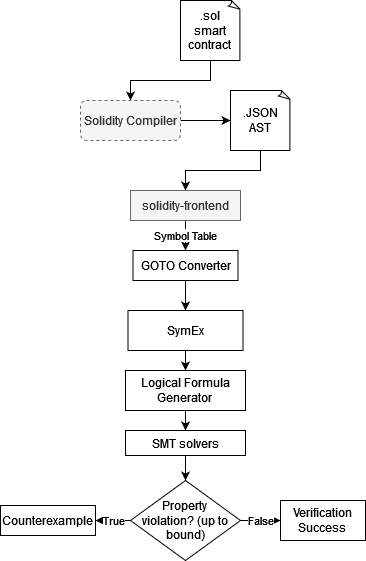
\includegraphics{ESBMC_process.png}
\caption{ESBMC's Verification Process \cite{song2022esbmc}}
\label{fig:ESBMC_process}
\end{figure}
\chapter{Methodology and Implementation}
\label{cha:methodology_and_implementation}

In this chapter, we outline the methodology and implementation of the project, focusing on the development of a benchmark suite of vulnerable smart contracts that cover a wide range of vulnerabilities listed in the Smart Contract Weakness Classification (SWC) Registry \cite{swc}. The purpose of this benchmark suite is to evaluate the capabilities and effectiveness of the ESBMC in detecting and mitigating smart contract vulnerabilities, ultimately contributing to the improvement of verification techniques and tools for smart contract security. By following a systematic and structured approach to create and analyze these vulnerable smart contracts, we aim to provide valuable insights into the performance of ESBMC and identify potential areas for enhancement, fostering the development of more secure and reliable blockchain ecosystems. The benchmark suite does not cover all of the SWC vulnerabilities, but we will discuss the remainder elsewhere, where a more analytical approach is required.


\section{SWC Registry Vulnerabilities}

In the following sections, we will look at each SWC vulnerability, discuss how to implement it in a smart contract, and evaluate how ESBMC tests it. The vulnerabilities have been listed in the order they appear in the SWC registry. 

\subsection{Function Default Visibility}
\label{sec:default_visibility}



The Function Default Visibility vulnerability (SWC-100) occurs when a function is not explicitly defined as public, internal, external, or private. The default function visibility, in this case, will be set to public which can be a security risk. For example, a function that is not intended to be called by other contracts can be called by other contracts if it is not explicitly defined as private.

An example of this vulnerability can be seen in fig. \ref{fig:default_visibility}

\begin{figure}
\begin{lstlisting}
    function defaultVisibility() {
        // This function is public by default.
    }
\end{lstlisting}
\caption{Extract from a vulnerable contract with Function Default Visibility vulnerability }
Source: esbmc-sbms/src/SWC-100/function\_default\_visibility.sol
\label{fig:default_visibility}
\end{figure}



Using recent solidity compilers (e.g. solc 0.8.0) the compiler itself will now output an error, as shown in fig. \ref{fig:default_visibility_error}, if a function is not explicitly defined as public, internal, external, or private. However, this is not the case for older versions of the compiler. This vulnerability would also be solved if a later vulnerability, SWC-102 (discussed in \ref{sec:outdated_compiler}), is implemented.
Since the vulnerability occurs when the contract is compiled using an older version of the compiler, when we check the AST of the contract, the function's default visibility will have already been set to public. Therefore, ESBMC will not be able to detect this vulnerability as it may not be able to distinguish between a function that is deliberately public or not.
\begin{figure}
\begin{lstlisting}
Error: No visibility specified. Did you intend to add "public"?
\end{lstlisting}
\caption{Error message from solc compiler when not setting function visibility}
\label{fig:default_visibility_error}
\end{figure}

\subsection{Integer Overflow and Underflow}
\label{sec:integer_overflow}



The Integer Overflow and Underflow vulnerability (SWC-101) occurs when an arithmetic operation results in a value greater than the maximum value for its type or less than the minimum value for its type. This error can lead to unexpected behavior and security vulnerabilities. For example, an integer overflow can bypass access vulnerable control checks. 

An example of this vulnerability can be seen in fig. \ref{fig:integer_overflow_underflow}

\begin{figure}
\begin{lstlisting}
//SPDX-License-Identifier: GPL-2.0
pragma solidity ^0.8.0;

contract IntegerOverflowUnderflow {
    uint256 public counter = 0;

    function increment() public {
        counter += 1;
    }

    function decrement() public {
        counter -= 1;
    }

    function instanceOfIntegerOverflow() public {
        uint256 max = 2**256 - 1;
        uint256 overflow = max + 1;
    }

    function instanceOfIntegerUnderflow() public {
        uint256 min = 0;
        uint256 underflow = min - 1;
    }
}
\end{lstlisting}
\caption{Example from a vulnerable contract with Integer Overflow vulnerability }
Source: esbmc-sbms/src/SWC-101/integer\_overflow\_underflow.sol
\label{fig:integer_overflow_underflow}
\end{figure}



ESBMC is effectively able to check for this vulnerability in solidity smart contracts.

\subsection{Outdated Compiler Version}
\label{sec:outdated_compiler}

The Outdated Compiler Version vulnerability (SWC-102) means that a legacy compiler version is used to compile the smart contract. This can lead to security vulnerabilities, especially if there are known vulnerabilities in the compiler version. For example, a compiler version that is vulnerable to tx.orign attacks can lead to a contract being exploited, despite the vulnerability largely being fixed in later versions of the compiler.

An example of this vulnerability can be seen in fig. \ref{fig:outdated_compiler_version}

\begin{figure}
\begin{lstlisting}
//SPDX-License-Identifier: GPL-2.0
pragma solidity 0.4.13;
\end{lstlisting}
\caption{Example from a vulnerable contract with Outdated Compiler Version vulnerability }
Source: esbmc-sbms/src/SWC-102/outdated\_compiler\_version.sol
\label{fig:outdated_compiler_version}
\end{figure}



As it stands, ESBMC does not check for this vulnerability. However, it is possible to implement this vulnerability by checking the compiler version used to compile the smart contract as the AST does explicitly state the version of the solidity compiler used. If the compiler version is outdated, then it would be considered to be vulnerable. However this would entail cultivating either a list of outdated compiler versions or a list of compiler versions that are vulnerable to known vulnerabilities. This is inherently a challenge since this list would need to be updated regularly, and it is not clear how to determine which compiler versions are vulnerable to which vulnerabilities.\\
ESBMC-Solidity is still in early stages of development as it stands and currently only supports checking individual functions, as opposed to the entire contract, as is possible in the clang frontend for example. This is a limitation which will be addressed many times in this report since many vulnerabilities fall outside of functions. 

\subsection{Floating Pragma}
\label{sec:floating_pragma}

The Floating Pragma vulnerability (SWC-103) occurs when the compiler version is not explicitly defined in the smart contract. This vulnerability is inherently similar to the Outdated Compiler Version vulnerability (SWC-102) as it can lead to security vulnerabilities, especially if there are known vulnerabilities in the compiler version. For example, a specific compiler version may have a known vulnerability that is fixed in a later version of the compiler or does not yet exist in an earlier version. If this specific compiler version is used to compile the smart contract, then the contract may be vulnerable to this known vulnerability.

An example of this vulnerability can be seen in fig. \ref{fig:floating_pragma}

\begin{figure}
\begin{lstlisting}
//SPDX-License-Identifier: GPL-2.0
pragma solidity ^0.8.0;
\end{lstlisting}
\caption{Example from a vulnerable contract with Floating Pragma vulnerability }
Source: esbmc-sbms/src/SWC-103/floating\_pragma.sol
\label{fig:floating_pragma}
\end{figure}

\begin{figure}
\begin{lstlisting}
      "id": 1,
      "literals": [
        "solidity",
        "^",
        "0.8",
        ".0"
      ]
\end{lstlisting}
\caption{AST of the contract with Floating Pragma vulnerability}
Source: esbmc-sbms/src/SWC-103/floating\_pragma.sol
\label{fig:floating_pragma_ast}
\end{figure}

Like the Outdated Compiler Version vulnerability (SWC-102), ESBMC does not have a feasible means to check for this issue, given that ESBMC-Solidity currently only supports checking individual functions. Once checking entire smart contracts is implemented, however (as is the case in the clang frontend), this vulnerability can be checked for by checking the compiler version used to compile the smart contract. If the version contains an element of the form \^, then it would be considered vulnerable, as seen in fig. \ref{fig:floating_pragma_ast}. 

\subsection{Unchecked Call Return Value}
\label{sec:unchecked_call_return_value}

The Unchecked Call Return Value vulnerability (SWC-104) occurs when the return value of a call is not checked. Execution therefore continues as if the call was successful, even if it was not. If the call was not successful, then the execution may be vulnerable to an attack, by breaking the contracts logic.

An example of this vulnerability can be seen in fig. \ref{fig:unchecked_return_value}. In this case a function call is made to the callee contract, and if that call were to fail, then the execution would return true. This could lead to a contract becoming vulnerable if a check is written as poorly as this, for example if the callee contract is used for an authentication check then it would not matter if the call failed, as the function would still return true.

\begin{figure}
\begin{lstlisting}
//SPDX-License-Identifier: GPL-2.0
pragma solidity ^0.8.0;

contract UncheckedReturnValue {
    function callchecked(address callee) public returns (bool) {
        require(callee.call());
        return true;
    }

    function callunchecked(address callee) public returns (bool) {
        callee.call();
        return true;
    }
}
\end{lstlisting}
\caption{Example from a vulnerable contract with Unchecked Call Return Value vulnerability }
Source: esbmc-sbms/src/SWC-104/unchecked\_return\_value.sol
\label{fig:unchecked_return_value}
\end{figure}

Although ESBMC-Solidity might not have direct support to check for unchecked return values, it is feasible to implement this capability as an extension. By analyzing the control flow and data dependencies within the smart contract code, the model checker could identify instances where external calls are made without validating the return values.

To implement this feature, developers could modify the ESBMC-Solidity tool to track external calls and analyze the subsequent operations to ensure that return values are checked before the execution proceeds. This may involve enhancing the symbolic execution engine and creating specific rules for return value checking. Once implemented, this feature could greatly contribute to the detection of unchecked return values vulnerabilities in Solidity smart contracts, improving their overall security and reliability

\subsection{Unprotected Ether Withdrawal}
\label{sec:unprotected_ether_withdrawal}

This vulnerability (SWC-105) can occur due to insufficient access controls. One common occurance of this vulnerability is when a contract has a constructor which is not correctly named, which means that the contract can be reinitialized, perhaps with a different owner which may have differing permissions, see Section. \ref{sec:incorrect_constructor_name}. The practical means of fixing a contract with a SWC-105 vulnerability is to ensure that withdrawals and other important functions can only be triggered successfully by some authorized parties. For ESBMC to check for this vulnerability, it would need to be able to check for the existence of access controls, which is not currently possible. ESBMC would also need to be able to detect when a Withdrawal is being made which is much more feasible.

\subsection{Unprotected Self-Destruct}
\label{sec:unprotected_self_destruct}

The Unprotected Self-Destruct vulnerability (SWC-106) occurs when a contract is able to be self-destructed without any sufficient restrictions. This can lead to the contract being exploited, as the contract can be destroyed by an attacker.

An example of this vulnerability can be seen in fig. \ref{fig:unprotected_self_destruct}

\begin{figure}
\begin{lstlisting}
//SPDX-License-Identifier: GPL-2.0
pragma solidity ^0.8.0;

contract UnprotectedSelfDestructInstruction {
    function destroyAnyone() public {
        selfdestruct(msg.sender);
    }
}
\end{lstlisting}
\caption{Example from a vulnerable contract with Unprotected Self-Destruct vulnerability }
Source: esbmc-sbms/src/SWC-106/unprotectedSelfDestruct.sol
\label{fig:unprotected_self_destruct}
\end{figure}

Currently, ESBMC does not support checking for this vulnerability at all in solidity since the ESBMC-Solidity frontend does not support checking for self-destruct instructions. An implementation may involve checking if a self-destruct instruction is found. If so, it would be considered vulnerable if the function it is held within is public. However, this is not an appropriate implementation since it is possible to have a self-destruct instruction in a private function, which is callable by a public function, which would be vulnerable and would not be detected by this implementation. The implementation would also incorrectly identify a contract as vulnerable if it has a self-destruct instruction in a public function that has sufficient access controls to the actual selfdestruct keyword. Nevertheless, this is a concerning vulnerability and should be addressed in the future.

\subsection{Reentrancy}
\label{sec:reentrancy}

Reentrancy (SWC-107) is a vulnerability which is easy to overlook while writing a smart contract. It occurs in Solidity smart contracts when a contract's function, while still in execution, is indirectly called again by an external contract before the initial function call is completed. This vulnerability can lead to unintended behavior and can potentially be exploited by attackers to manipulate the state of the contract or drain its funds.

The root cause of reentrancy vulnerability often lies in the inappropriate ordering of statements in a function. For instance, if a contract's function first transfers funds to an external address (using a low-level function like call) and then updates the internal state (such as the balance of the sender), an attacker might create a malicious contract that, when called by the vulnerable contract, recursively calls the original function before the state update is executed. This allows the attacker to repeatedly withdraw funds without the vulnerable contract realizing the depletion of its balance.

An example of this vulnerability can be seen in fig. \ref{fig:reentrancy}. This withdraw function is vulnerable to reentrancy because the balance of the sender is updated before the transfer is made. This means that if the transfer fails, the balance of the sender will still be updated. If the transfer is successful, the balance of the sender will be updated twice. This is because the transfer function will call the fallback function of the malicious contract, which will call the withdraw function again. This will result in the balance of the sender being updated twice, which is incorrect. Various techniques such as using a mutex locked varable or the "Checks-Effects-Interactions" pattern, can mitigate this vulnerability.

\begin{figure}
\begin{lstlisting}
// SPDX-License-Identifier: GPL-2.0
pragma solidity ^0.8.0;

contract Reentrancy {

    mapping (address => uint) public balances;

    function donate(address _to) public payable {
        balances[_to] += msg.value;
    }

    function withdraw(uint _amount) public {
        if (balances[msg.sender] >= _amount) {
            (bool result, ) = msg.sender.call{value: _amount}("");
            require(result);
            balances[msg.sender] -= _amount;
        }
    }

    function getBalance(address to) public view returns (uint) {
        return balances[to];
    }
}
\end{lstlisting}
\caption{Example from a vulnerable contract with Reentrancy vulnerability }
Source: esbmc-sbms/src/SWC-107/reentrancy.sol
\label{fig:reentrancy}
\end{figure}

ESBMC-Solidity can already check for reentrancy vulnerabilities \cite{salim2022esbmc}. SWC-107, in that case, is implemented successfully.

\subsection{State Variable Default Visibility}
\label{sec:state_variable_default_visibility}

The State Variable Default Visibility vulnerability (SWC-108) occurs when a state variable is not explicitly declared as public, private, or internal. This vulnerability means that the state variable is public by default, which can lead to unintended behavior. An attacker can exploit this vulnerability to manipulate the state of the contract or drain its funds. This vulnerability is fundamentally similar in nature to the Function Default Visibility vulnerability (SWC-103), which is discussed in section \ref{sec:default_visibility}.

An example of the vulnerability is seen in \ref{fig:state_variable_default_visibility} where the state variable d is internal by default. This may cause unintended behavior if another contract extends the contract. If the contract is extended by another contract, the state variable d will be accessible by the extended contract. This may lead to unintended behavior and can potentially be exploited by attackers to manipulate the state of the contract or drain its funds.

\begin{figure}
\begin{lstlisting}
    contract StateVariableDefaultVisibility {
        uint public a;
        uint internal b;
        uint private c;
        uint d;
    
        function f() public {
            a = 1;
            b = 2;
            c = 3;
            d = 4;
        }
    }
\end{lstlisting}
\caption{Example from a vulnerable contract with State Variable Default Visibility vulnerability }
Source: esbmc-sbms/src/SWC-108/state\_variable\_default\_visibility.sol
\label{fig:state_variable_default_visibility}
\end{figure}

Unlike in the case of the Function Default Visibility vulnerability, the solc compiler does not output an error when a state variable is not explicitly declared as public, private, or internal; instead it is internal by default, and there is no distinguishing marker in the AST to indicate that the state variable is internal by default or by purpose. This means that ESBMC-Solidity cannot check for this vulnerability at the moment, but this may be implemented in the solidity compiler and so may become unnecessary in the future.

\subsection{Unitialized Storage Pointer}
\label{sec:uninitialized_storage_pointer}

Uninitialized Storage Pointer (SWC-109) is a vulnerability that occurs when a storage pointer is not initialized. Therefore uninitialized local storage pointers can point to unexpected locations, leading to unintended behavior. This vulnerability has been resolved in Solidity 0.5.0, thus this vulnerability will be addressed sufficiently if the outdated compiler version vulnerability (SWC-102) discussed in section \ref{sec:outdated_compiler} is also addressed.

\subsection{Assert Violation}
\label{sec:assert_violation}

Well-implemented code should not contain any assert violations. There are two reasons an assertion failure can occur. Either a bug in the contract allows it to enter an invalid state, or the assert statement is used incorrectly. The Assert Violation vulnerability (SWC-110) occurs when an assert statement is used incorrectly. 

This vulnerability is shown in \ref{fig:assert_violation}. The assert statement is used incorrectly in this example. The assert statement is used to check if false is true, which is always false. This means that the assert statement will always fail, and the contract will always revert. 

\begin{figure}
\begin{lstlisting}
    function foo() public pure {
        assert(false);
    }
\end{lstlisting}

\begin{lstlisting}
Counterexample:

State 1 file assert_violation.sol line 17 function foo thread 0
----------------------------------------------------
Violated property:
  file assert_violation.sol line 17 function foo
  assertion
  0
\end{lstlisting}
\caption{Example from a vulnerable contract with Assert Violation vulnerability }
Source: esbmc-sbms/src/SWC-110/assert\_violation.sol
\label{fig:assert_violation}
\end{figure}

ESBMC-Solidity is capable of checking for this vulnerability, as seen in \ref{fig:assert_violation}, providing a counterexample that shows the assert statement is violated. Thus this vulnerability is implemented successfully.

\subsection{Use of Deprecated Solidity Functions}
\label{sec:use_of_deprecated_solidity_functions}

For a language to maintain backward compatibility with older versions of itself, it is necessary not to change the functionality of existing functions as they are made obsolete or deemed insecure. This way, people with experience using the older language versions can be aware of the changes and update their code accordingly. However, this can lead to the creation of new functions similar to the old ones but with different functionality. This can lead to confusion and cause developers to use the old functions, leading to unintended and insecure behavior. This vulnerability is known as the Use of Deprecated Solidity Functions vulnerability (SWC-111). 

An example of some use of deprecated solidity functions can be found in fig. \ref{fig:deprecated_solidity_functions}. 

\begin{figure}
\begin{lstlisting}
    function suicideContract() public {
        // Use selfdesturct(address) instead
        suicide(msg.sender);
    }

    function callcode() public {
        // Use call() instead
        msg.sender.callcode();
    }

    function getBlockHash(uint x) public returns(bytes32) {
        return block.blockhash(x);
    }

    function hash(uint x) public returns(bytes32) {
        return sha3(x);
    }

    function getGas() public returns(uint){
        return msg.gas;
    }

    function useThrow() public {
        throw;
    }

    function set_variables() public {
        constant c = 1;
        var v = 2;
    }
\end{lstlisting}
\caption{Examples of deprecated solidity functions}
\label{fig:deprecated_solidity_functions}
\end{figure}

Fortunately, the use of these deprecated functions will cause recent versions of the solidity compiler to throw an error. Therefore this is not a vulnerability ESBMC-Solidity would need to check. However, it would still be possible for a contract that is compiled with an outdated compiler (as discussed in section \ref{sec:outdated_compiler}) to still use these now insecure functions. Therefore, once again, it emphasizes implementing (SWC-102). However this vulnerability could never be fully resolved as functions will always be deprecated and replaced with new ones as time passes on.

\subsection{Delegatecall to Untrusted Callee}
\label{sec:delegatecall_to_untrusted_callee}

This vulnerability (SWC-112) occurs when a contract calls a function using delegatecall to an untrusted contract. The method \verb|delegatecall| is a variant of a message call, which only differs where the code at the target address is exectued within the contract it is called from (the caller) without changing the values of \verb|msg.sender| and \verb|msg.value|. This should be used sparingly as it allows smart contracts to dynamically load code from untrusted addresses after compilation, and many elements, for example the balance of the contract, can be manipulated by the callee. 

ESBMC-Solidity's capacity to check for this vulnerability is limited, since the vulnerability is more of a bad practice in nature and there are many instances where it is acceptable to use delegatecall. For example, it is acceptable to use delegatecall when calling a library function. However, it is not acceptable to use delegatecall when calling a function from an untrusted contract. Therefore, there is no feasible way to check for this vulnerability in ESBMC-Solidity, as it would involve analyzing whether or not a callee is trusted, which is not feasible. 

\subsection{DoS with Failed Call}
\label{sec:dos_with_failed_call}

External calls will fail sometimes, for example when the called contract runs out of gas. This can be exploited to cause a denial of service. This vulnerability is known as the DoS with Failed Call vulnerability (SWC-113). For example if a contract calls a function in another contract, and the function in the other contract runs out of gas, the contract may revert. This means that the contract will not be able to continue executing, and this may mean that neccesary tasks are not completed.

In figure \ref{fig:failed_call}, the function failLoop will terminate if any of the calls to send fail. Thus ending the loop prematurely and in this case, not sending all the funds to the addresses. 


\begin{figure}
\begin{lstlisting}
    function failLoop() public {
        for (uint i = 0; i < _addresses.length; i++) {
            require(_addresses[i].send(_balances[_addresses[i]]));
        }
    }
\end{lstlisting}
\caption{Example from a vulnerable contract with DoS with Failed Call vulnerability}
\label{fig:failed_call}
Source: esbmc-sbms/src/SWC-113/DoS\_with\_failed\_call.sol
\end{figure}

Currently when testing for this vulnerability, ESBMC-Solidity would abort the analysis, citing issue \verb|terminate called after throwing an instance of 'nlohmann::detail::type_error'|. 

\subsection{Authorization through tx.origin}
\label{sec:authorization_through_tx.origin}

Similarly to the Use Of Deprecated Solidity Functions vulnerability (section. \ref{sec:use_of_deprecated_solidity_functions} SWC-111), the use of \verb|tx.origin| for authorization is also deprecated. The \verb|tx.origin| variable is the address of the account that sent the transaction. If an authorized account calls into a malicious contract that calls back into the main contract using \verb|tx.origin|, the malicious contract will be able to call functions that it is not authorized to call. This vulnerability is known as the Authorization through tx.origin vulnerability (SWC-115). 

An example of this vulnerability can be found in figure \ref{fig:tx.origin}. The function sendTo will only allow the owner of the contract to send ether to another address. However, if the owner calls a malicious contract that calls back into the main contract using \verb|tx.origin|, the malicious contract will be able to call the function sendTo and send ether to any address. 

\begin{figure}
\begin{lstlisting}
    function sendTo(address payable _to) public {
        require(tx.origin == owner);
        _to.transfer(1 ether);
    }
\end{lstlisting}

\begin{lstlisting}
Checking function sendTo ...
    - Pattern-based checking: SWC-115 Authorization through tx.origin
   checking function body stmt 0
  ERROR: Found vulnerability SWC-115 Authorization through tx.origin
  ERROR: VERIFICATION FAILED
\end{lstlisting}
\caption{Example from a vulnerable contract with Authorization through tx.origin vulnerability}
\label{fig:tx.origin}
Source: esbmc-sbms/src/SWC-115/authorization\_through\_tx\_origin.sol
\end{figure}

This vulnerability is very common and a simple fix for ESBMC-Solidity which has already been implemented, as it is a simple pattern-based check \cite{salim2022esbmc}.

\subsection{Block Values as a Proxy for Time}
\label{sec:block_values_as_a_proxy_for_time}

The Solidity vulnerability "Block Values as a Proxy for Time" arises when developers rely on block properties, such as block numbers or block timestamps, to measure time durations or control the execution flow of a smart contract. This practice can lead to potential security risks and unintended behaviors due to the inherent variability and manipulability of block-related properties.

Block numbers and timestamps can be influenced by miners to a certain extent, allowing for potential exploitation. For example, a miner might manipulate the block timestamp to impact the outcome of a time-based condition within a smart contract. Using block values as a proxy for time can also result in imprecision due to the variable nature of block times, which might deviate from the expected average block time on the network.

To mitigate this vulnerability, developers should avoid using block properties to control critical time-sensitive operations in smart contracts. Instead, they should consider using alternative mechanisms that are less susceptible to manipulation, such as external time oracles or predefined intervals that do not depend on block values. By ensuring that smart contracts handle time-related operations securely, developers can prevent potential exploitation and maintain the reliability and trustworthiness of the contract.

ESBMC-Solidity can check for this vulnerability by checking if the block number or timestamp is used in a conditional statement. If it is, then the vulnerability is present. This is not yet implemented in ESBMC-Solidity. This is not exhaustive, as there are many other ways to use block values as a proxy for time, but it is a good start. For example in \ref{fig:block_values_as_a_proxy_for_time} the function lockEth uses the block number to determine when the user can withdraw their funds. The line \verb|...unlockBlock = block.number + (_time / 14)| sets the unlockBlock to the current block number plus the time in seconds divided by 14, but future logic involving the unlockBlock variable is not checked. This means that an attacker could use the unlockBlock variable in a conditional statement that ESBMC-Solidity does not check even under this implementation.

\begin{figure}
\begin{lstlisting}
function lockEth(uint _time, uint _amount) public payable {
        require(msg.value == _amount, 'must send exact amount');
        users[msg.sender].unlockBlock = block.number + (_time / 14);
        users[msg.sender].amount = _amount;
}
\end{lstlisting}
\caption{Example from a vulnerable contract with Block Values as a Proxy for Time vulnerability}
Source: \url{https://swcregistry.io/docs/SWC-116#time_locksol} \cite{timelock}
\label{fig:block_values_as_a_proxy_for_time}
\end{figure}

\subsection{Incorrect Constructor Name}
\label{sec:incorrect_constructor_name}

Over the period solidity has been developed, there have been many ways to define a constructor for an object. The most common way is to define a function with the same name as the contract, but this is not the only way. In solidity, a constructor can be defined by using the \verb|constructor| keyword, or by defining a function with the same name as the contract. The \verb|constructor| keyword was introduced in Solidity 0.4.22, and the function with the same name as the contract was deprecated in Solidity 0.4.22. It can therefore be a vulnerability to incorrectly define a constructor (SWC-118).

As seen in figure \ref{fig:incorrect_constructor_name}, the more recent versions of the solidity compiler will output an error if a function with the same name as the contract is defined. However, the older versions of the solidity compiler will not output an error, and will instead define the function with the same name as the contract as the constructor. This means that the function with the same name as the contract will be called when the contract is deployed, and not when the contract is instantiated. This can lead to unexpected behavior, and is a security vulnerability. Once again, this is another issue that can be solved by solving the Outdated Compiler version vulnerability (section \ref{sec:outdated_compiler_version} SWC-101) or the Floating Pragma vulnerability (section \ref{sec:floating_pragma} SWC-102).

This does not however solve all the possible ways of reaching this vulnerability. For example, if a developer is used to constructors' implementation previous to Solidity 0.4.22, they might define a function with the same name as the contract and additionally make a spelling error leading to the creation of a public function which has some capabilities of a constructor (such as being able to receive ether). This is not a vulnerability, but it is a common mistake that developers make. Handling this case is not trivial but is a lower priority issue than other vulnerabilities.

\begin{figure}
\begin{lstlisting}
Error: Functions are not allowed to have the same name as the
contract. If you intend this to be a constructor, use
"constructor(...) { ... }" to define it. 
\end{lstlisting}
\caption{Error outputted when using a function with the same name as the contract}
\label{fig:incorrect_constructor_name}
\end{figure}

\subsection{Shadowing State Variables}
\label{sec:shadowing_state_variables}

When Inheritance is used in Solidity, the child contract inherits all the state variables and functions from the parent contract. However, if the child contract defines a state variable with the same name as a state variable in the parent contract, the child contract's state variable will shadow the parent contract's state variable. There would then be a different state variable with the same name in the child contract and the parent contract (SWC-119). 

Since inheritance is not a feature that ESBMC-Solidity is capable of checking, given that the object oriented features of Solidity are not yet fully supported, this vulnerability is not yet implemented in ESBMC-Solidity. However, this is a vulnerability that is very common and should be implemented in the future. However the more recent solidity compilers will output a warning if a state variable is shadowed, so this vulnerability can be mitigated by using a more recent version of the solidity compiler (section \ref{sec:outdated_compiler_version} SWC-101).

\subsection{Weak Sources of Randomness from Chain Attributes}
\label{sec:weak_sources_of_randomness_from_chain_attributes}

There are many reasons that it is feasible that a developer may choose to involve randomness in a smart contract (SWC-120). For example, the contract may have a lottery, a game, or a need for random numbers for security. Therefore it is important that the randomness is secure and cannot be manipulated by an attacker. It is difficult to create a strong source of randomness in Ethereum as a large amount of the randomness is determined by the miners. However, there are some ways to create a strong source of randomness, by using a trusted randomness oracle \cite{allemann2021randomness} or a commitment scheme. Ethereum does however contain some weak sources of randomness that can be used in smart contracts. These weak sources of randomness are the block hash, the block number, and the block timestamp. These are all weak sources of randomness because they can be manipulated by miners, and thus should not be used in smart contracts as a source of randomness. Solidity does contain a \verb|prevrandao| which replaces the \verb|difficulty| field in the block header.

This is not a vulnerability that ESBMC-Solidity could feasibly check for, as it would require the ability to understand the intention of a program and whether or not the program is using the \verb|prevrandao|, \verb|timestamp| field as a source of randomness, or as other intended uses.

\subsection{Missing Protection against Signature Replay Attacks}
\label{sec:missing_protection_against_signature_replay_attacks}

Signature replay attacks are a type of attack that can be used to steal funds from a smart contract. In a signature replay attack, an attacker can use a signature that was intended for a smart contract to only be used a single time, multiple times. For example, suppose they choose to make a particular transaction, say a withdrawal, and receive a signature for verification. In that case, they can use that signature multiple times to withdraw the funds from the smart contract. A lack of this kind of protection is a vulnerability (SWC-121). To avoid this vulnerability, you could, for example, store every message hash used to withdraw funds from the smart contract and check that the message hash has not been used before.

ESBMC-Solidity is primarily focused on detecting vulnerabilities that arise due to incorrect implementation or logical flaws in the contract's code. It is designed to verify safety properties, such as absence of overflows, underflows, and out-of-bounds memory access, as well as user-defined properties and assertions. However, signature replay attacks are not directly related to implementing the smart contract's code itself but are more concerned with the context and sequence of transactions. These attacks involve a malicious actor reusing a valid signature from a previous transaction to execute the same operation without the consent of the original signer. This is a vulnerability that does not have a straightforward solution, and thus is not a vulnerability that ESBMC-Solidity can feasibly check for.

\subsection{Lack of Proper Signature Verification}
\label{sec:lack_of_proper_signature_verification}

The Lack of Proper Signature Verification vulnerability (SWC-122) occurs when a smart contract does not correctly validate digital signatures, enabling attackers to forge or manipulate signatures and gain unauthorized access or perform actions on behalf of other users. This vulnerability can lead to severe security breaches and allow malicious actors to compromise the integrity of a smart contract.

Digital signatures are commonly used in smart contracts to authenticate users and prove that they have authorized specific actions or transactions. The Ethereum platform provides a built-in mechanism, the Ethereum-Signed Message (EIP-712), which allows users to sign messages off-chain. This technique reduces the on-chain computational load and gas costs associated with verifying signatures. The built-in \verb|ecrecover| function provided by Solidity can verify the signer's address from a given message hash and its corresponding signature, and using alternative signature verification schemes is not recommended.

Figure \ref{fig:signature_verification} shows an example of good practice for signature verification. This contract implements a function that verifies the signature of a message hash. The function first splits the signature into its three components: the recovery ID, the R component, and the S component. It then uses the \verb|ecrecover| function to recover the signer's address from the message hash and the signature. The function returns the recovered address.


\begin{figure}
\begin{lstlisting}
pragma solidity ^0.8.0;

contract SignatureVerification {
    function verifySignature(bytes32 messageHash,
    bytes memory signature) public pure returns (address) {
        uint8 v;
        bytes32 r;
        bytes32 s;
        
        (v, r, s) = splitSignature(signature);
        return ecrecover(messageHash, v, r, s);
    }

    function splitSignature(bytes memory sig)
    internal pure returns (uint8 v, bytes32 r, bytes32 s) {
        require(sig.length == 65, "Invalid signature length");

        assembly {
            r := mload(add(sig, 0x20))
            s := mload(add(sig, 0x40))
            v := byte(0, mload(add(sig, 0x60)))
        }
    }
}
\end{lstlisting}
\caption{Example of a contract that verifies signatures}
\label{fig:signature_verification}
\end{figure}

ESBMC-Solidity currently does not check for SWC-122. Some pattern-based checks could be implemented to detect this vulnerability, but it's unclear how it would be possible to make an exhaustive check for this vulnerability.

\subsection{Requirement Violation}
\label{sec:requirement_violation}

The Require Violation vulnerability (SWC-123) occurs when a smart contract does not correctly validate the input parameters of a function. A \verb|require()|, \verb|revert()| or \verb|assert| statement should only fail if there is a bug in the external contract that is called. In this case, since ESBMC solidity cannot detect bugs in external contracts, it is not possible to detect errors in this manner. However this is a vulnerability ESBMC can verify very well.  Bounded model checking is used to symbolically execute the smart contract and explore its possible execution paths. During this process, ESBMC-Solidity evaluates the conditions specified in require() statements and determines whether they can be violated under any circumstances. If a requirement violation is detected, ESBMC-Solidity will report it, usually with a counterexample showing the input values or contract state that caused the violation \cite{salim2022esbmc}.
\subsection{Write to Arbitrary Storage Location}
\label{sec:write_to_arbitrary_storage_location}

It's crucial for a smart contract to store data in a secure manner. Data is stored persistently in a storage location with a key or an address for the sake of the EVM level. It is therefore essential that unauthorized users or unauthorized contract accounts do not have write access to the storage location. This vulnerability (SWC-124) occurs when a smart contract allows unauthorized users to write to arbitrary storage locations, circumventing the authorization checks and corrupting the stored data. This vulnerability can lead to important information being overwritten or deleted.

\begin{figure}
\begin{lstlisting}
    function pushToArray(uint value) public {
        array.push(value);
    }

    function pushToArraySafe(uint value) public {
        require(msg.sender == owner);
        array.push(value);
    }
\end{lstlisting}
\caption{Example of a contract that includes a function that allows unauthorized users to write to arbitrary storage locations, and a function that prevents unauthorized users from writing to arbitrary storage locations}
\label{fig:write_to_arbitrary_storage_location}
\end{figure}

Figure \ref{fig:write_to_arbitrary_storage_location} shows an example of a contract that includes a function that allows unauthorized users to write to arbitrary storage locations, and a function that prevents unauthorized users from writing to arbitrary storage locations. The first function, \verb|pushToArray|, allows any user to push a value to the array. The second function, \verb|pushToArraySafe|, only allows the owner of the contract to push a value to the array. The second function is a safer implementation of the first function, as it prevents unauthorized users from writing to arbitrary storage locations. This vulnerability is based off of a common vulnerability where insufficient authorization checks are performed, which is a common factor in many of these vulnerabilities. ESBMC-Solidity could not feasibly check for this vulnerability since it would require checking for all possible authorization checks, which is not currently feasible.

\subsection{Insufficient Gas Griefing}
\label{sec:insufficient_gas_griefing}

The Insufficient Gas Griefing vulnerability (SWC-126) arises when a smart contract relies on the assumption that an externally called contract function will always have enough gas to execute successfully. If a contract does not account for the possibility of the called function running out of gas, it may result in unexpected behavior or unintended consequences, potentially compromising the security and integrity of the smart contract.

In Ethereum, gas is used as a measure of computational effort required to execute an operation. When a function runs out of gas during execution, it reverts all changes made during that function call, as if it never occurred. A malicious actor could exploit the Insufficient Gas Griefing vulnerability by intentionally providing insufficient gas to the called function, causing it to fail and potentially disrupting the normal operation of the smart contract. This vulnerability is very much a runtime vulnerability, but once again we are considering appropriate access control and insufficient checking of return values, as discussed in Section. \ref{sec:unchecked_call_return_value}.


\subsection{Typographical Error}
\label{sec:typographical_error}

Typographical errors are a common cause of vulnerabilities in smart contracts. This vulnerability (SWC-128) occurs when a smart contract contains a typo that causes the contract to behave differently than intended. This vulnerability can lead to severe security breaches and allow malicious actors to compromise the integrity of a smart contract. For example, a typo in a function name can cause the function to be called unintentionally, or a typo in a variable name can cause the variable to be assigned a different value than intended. The example in the project, fig \ref{fig:typographical_error}, shows a function that is supposed to increment a variable, but instead reinitializes the variable to 0. This is a typographical error that can lead to a vulnerability. The unary operator in this case however, has been disallowed in Solidity 0.8.0, so this example is no longer valid. As with many of the other vulnerabilities in the SWC registry, the solidity compiler has been updated with specific cases of common pitfalls, and so implementing Outdated Compiler (\ref{sec:outdated_compiler} SWC-102) is a good way to avoid this vulnerability. However it is not feasible for ESBMC-Solidity to check for all possible typographical errors, so this vulnerability is not currently checked, and it would not be feasible to implement.

\begin{figure}
\begin{lstlisting}
    function incrimentVulnerable() public{
        i =+1; // This reinitializes the variable
    }
\end{lstlisting}
\caption{An extract from a contract that contains a typographical error}
\label{fig:typographical_error}
\end{figure}

\subsection{Presence of unused variables}
\label{sec:presence_of_unused_variables}

Despite being listed in the SWC Registry (as SWC-131), the presence of unused variables is not a security risk and as such has a lower priority than other issues in this registry. However, it is still a good practice to remove unused variables from a smart contract, as they can cause confusion and make the code harder to read and understand. This would however be a simple check as the AST Json file contains information about the variables used in the contract, and when they're used. This could be implemented as a pattern-based check, and would be a good first issue for a new contributor. The solidity compiler already checks for unused local variables, and will throw warnings if it finds any, for example: \verb|Warning: Unused local variable.|

\subsection{Unexpected Ether balance}
\label{sec:unexpected_ether_balance}

If a smart contract functions on having an exact amount of Ether in its balance, then it is important that the contract does not receive any additional Ether. This vulnerability (SWC-132) occurs when a smart contract receives Ether that it does not expect. This vulnerability can lead to severe security breaches and allow malicious actors to compromise the integrity of a smart contract. For this reason it is imperative that no smart contract relies on having an exact amount of Ether balance. As seen in the example in fig \ref{fig:unexpected_ether_balance}, the contract in this example relies on having an exact amount of Ether balance (8 Ether). If the contract recieves more Ether then the function would be unable to continue. This vulnerability is not currently checked by ESBMC-Solidity. Still, it would be possible to implement a pattern-based check for this vulnerability, throwing an error whenever a balance is placed in a conditional function or if statement.

\begin{figure}
\begin{lstlisting}
    function g() public payable {
        require(msg.value == 8);
        require(msg.sender.balance == 8);
    }
\end{lstlisting}
\caption{An extract from a vulnerable contract that relies on having an exact amount of Ether balance}
\label{fig:unexpected_ether_balance}
\end{figure}

\subsection{Hash Collisions with Multiple Variable Length Arguments}
\label{sec:hash_collisions_with_multiple_variable_length_arguments}

Hash Collisions With Multiple Variable Length Arguments (SWC-133) occurs when a smart contract function uses \verb|abi.encodePacked()| with multiple variable-length arguments, which, under certain circumstances, can result in hash collisions. This can happen because \verb|abi.encodePacked()| concatenates all elements in order, regardless of whether they belong to an array or not. As a result, elements can be moved between arrays, and as long as they maintain the same order, the encoding will remain the same. In situations where signature verification is involved, an attacker can exploit this vulnerability by modifying the position of elements in a previous function call, effectively bypassing authorization.

To remediate this vulnerability, it is crucial to ensure that matching signatures cannot be achieved using different parameters when using \verb|abi.encodePacked()|. Developers can do this by either restricting user access to the parameters used in abi.encodePacked() or by using fixed-length arrays. Alternatively, developers can use \verb|abi.encode()| instead, which properly encodes the data structure and its length information, preventing ambiguous concatenation.

Additionally, it is recommended to implement replay protection (see SWC-121) in the smart contract. However, it is essential to note that an attacker could still attempt to bypass this protection by front-running the transaction. By adhering to these best practices, developers can mitigate the risk of SWC-133 vulnerabilities and ensure the security and integrity of their smart contracts.

When checking this vulnerability, ESBMC-Solidity would need to check for any usage of \verb|abi.encodePacked()| with multiple variable-length arguments. This would be a simple pattern-based check, which is not yet implemented in ESBMC-Solidity.

\subsection{Message call with hardcoded gas amount}
\label{sec:message_call_with_hardcoded_gas_amount}

Many smart contracts use functions with hardcoded gas amounts (SWC-134), for example the \verb|transfer()| function has a fixed amount of 2300 gas, but it is advised to change these gas amounts, as they are one of many factors that can lead to a reentrancy attack (see section \ref{sec:reentrancy}). This vulnerability (SWC-134) occurs when a smart contract function uses a hardcoded gas amount. The EVM instructions invovled may change during the execution of the contract, and so the hardcoded gas amount may not be enough to execute the function. For this reason it's best to avoid the \verb|transfer()| and \verb|send()| functions. This vulnerability is not currently checked by ESBMC-Solidity. Still, it would be possible to implement a pattern-based check for this vulnerability, throwing an error whenever a hardcoded gas amount is used, but significantly easier will be to simply flag any usage of the \verb|send()| and \verb|transfer()| as vulnerable - as per the advice given after EIP-1884 \cite{eip-1884}. However currently the ESBMC-Solidity tool does not yet have the ability to test \verb|adress payable| type variables, so this would need to be implemented first \cite{lawley2023esbmc}.


\subsection{Unencrypted Private Data On-Chain}
\label{sec:unencrypted_private_data_on_chain}

Unencrypted Private Data On-Chain (SWC-135) occurs when a smart contract stores private data on-chain without encrypting it. This can lead to a variety of security issues, including the possibility of data theft and the exposure of sensitive information. This vulnerability can be mitigated by encrypting the data before storing it on-chain. This can be done using a variety of encryption algorithms, such as AES, RSA, or ECC. Additionally, it is recommended to use a key management system to store the encryption keys. This will ensure that the keys are not stored on-chain, and that they are not exposed to malicious actors. Simply setting a variable as private is not sufficient, as seen with \_privateVariable in the example in fig \ref{fig:unencrypted_private_data_on_chain}. This variable is still stored on-chain, and can be accessed by anyone with access to the contract. To prevent this vulnerability, it is important to encrypt the data before storing it on-chain. Running ESBMC on either function in the example in fig \ref{fig:unencrypted_private_data_on_chain} will incorrectly result in a successful verification, (the function \verb|setPrivateVariable()| 's output is shown in fig \ref{fig:unencrypted_private_data_on_chain}). This could be implemented by checking if a variable is private and is being returned or otherwise being made visible on chain, and throwing an error if this is the case.

\begin{figure}
\begin{lstlisting}
//SPDX-License-Identifier: GPL-2.0
pragma solidity ^0.8.0;

contract ReadablePrivateVariables {
    uint256 private _privateVariable = 42;

    function setPrivateVariable(uint256 value) public {
        _privateVariable = value;
    }

    function getPrivateVariable() public view returns (uint256) {
        return _privateVariable;
    }
}
\end{lstlisting}
\begin{lstlisting}
ESBMC version 7.1.0 64-bit x86_64 linux
Target: 64-bit little-endian x86_64-unknown-linux with esbmclibc
Parsing
Converting
Done conversion of intrinsics...
Checking function setPrivateVariable ...
  - Pattern-based checking: SWC-115 Authorization through tx.origin
 checking function body stmt 0
Generating GOTO Program
GOTO program creation time: 0.131s
GOTO program processing time: 0.000s
Starting Bounded Model Checking
Symex completed in: 0.000s (12 assignments)
Slicing time: 0.000s (removed 12 assignments)
Generated 0 VCC(s), 0 remaining after simplification (0 assignments)
BMC program time: 0.000s

VERIFICATION SUCCESSFUL
\end{lstlisting}
\caption{An extract from a vulnerable contract that stores private data on-chain without encrypting it}
\label{fig:unencrypted_private_data_on_chain}
\end{figure}

\subsection{Other vulnerabilities}
\label{sec:other_vulnerabilities}

The following SWC \cite{swc} vulnerabilities were not addressed in this paper, but are still important to consider when developing smart contracts. These vulnerabilities are:

\begin{itemize}
    \item \textbf{SWC-114: Transaction Order Dependence: }I determined that this vulnerability would be beyond the scope of this project to discuss.
    \item \textbf{SWC-117: Signature Malleability: } This vulnerability was not one I was willing to investigate further as I do not believe I have the necessary knowledge to do so.
    \item \textbf{SWC-125: Incorrect Inheritance Order: }With the current implementation of ESBMC-Solidity, the evaluation of inheritance does not seem like a priority, as the current Object-Oriented features of solidity implementations are not yet fully supported. 
    \item \textbf{SWC-130: Right-To-Left-Override Control Character: } There are very few legitimate uses for this character, and should be avoided as much as possible. This vulnerability is not currently checked by ESBMC-Solidity, but could be implemented by checking for the presence of this character in the source code, and throwing an error if it is found.
    \item \textbf{SWC-135: Code with No Effects: } This issue has been discussed in the solidity compiler github \cite{solidity_issue_7118}, and this may not be an appropriate place to discuss this issue.
\end{itemize}

\bibliography{refs.bib}

\bibliographystyle{abbrv}
%% the bibliography style determines the format  in which both citations and references are printed,
%% other possible values are plain and abbrv
%%
%% If you want more control of the format of your citations you might want to take a look at
%% natbib.sty, which should be part of any standard LaTeX installation
%%
%% University regulations simply require that your citation style be consistent, so see what style
%% your supervisor recommends.

% Appendices start here

\appendix
\chapter{Appendix Title}



\section{Example First Section}

TODO:




\section{Output}

TODO:


\end{document}
